\chapter{The \gerda\ experiment}\label{chap:gerda}

The GERmanium Detector Array (\gerda) experiment has been proposed in
2004~\cite{gerda-proposal} to search for neutrinoless double-beta decay with high-purity
germanium detectors enriched in the \gesix\ double-beta emitter. The proposal lies in the
path opened by the Heidelberg-Moscow (\hdm)~\cite{Klapdor2001} and
\igex~\cite{Aalseth2002} experiments, aiming to develop the germanium technology towards
large-scale, \bkgfree\ experimental conditions that could tackle the scale of
$\mathcal{O}(10^{26})$~yr sensitivity on the neutrinoless double-beta decay half-life. The
\gerda\ data taking officially ended in December 2019 after hitting the target total
\bkgfree\ exposure of 100~\kgyr\ and establishing itself as the leading experiment in the
field in terms of lowest background level ever achieved around \qbb~\cite{Agostini2019a}.

\marginnote{\gerda\ \\ phases}
Since the start of the data taking in 2008 the experiment, located in hall~A of the Gran
Sasso National Laboratories (LNGS) in Italy, has been running through two distinct
experimental phases (\phaseone\ and \phasetwo). Detectors from the former \hdm\ and
\igex\ experiments (of semi-coaxial geometry) along with newly produced diodes (of BEGe
geometry type, shorthand for Broad Energy Germanium detectors) were deployed bare into
liquid argon (LAr) during \phaseone, following a suggestion by \fillme, for a total amount
of 21.3~kg of germanium. \phaseone\ ended in June 2013 with a total exposure of
21.6~\kgyr\ and a background index in the region of interest of \pIbi~\cite{Agostini2016}.
Short after the upgrade works for \gerda\ \phasetwo\ started: a new event veto system
based on the LAr scintillation light was installed along with an additional 20~kg of
BEGe-type detectors.  The newly designed veto system allowed for a significant reduction
of the background index (BI) down to the \vctsper\ scale, allowing \gerda\ to seamlessly
run in \bkgfree\ conditions for its full second experimental phase and surpass the
\powtenyr{26} threshold sensitivity~\cite{Agostini2019a} in April 2018. Data taking was
then stopped again to permit a third hardware upgrade, during which another \fillme~kg of
enriched germanium in the form of four inverted-coaxial geometry detectors were deployed
and the LAr veto system improved in detection efficiency in the space between the
detectors. This last part of \phasetwo, which will be referred as \phasetwop in the
following, ended in December 2019 after collecting the total exposure of \fillme~\kgyr\
and establishing the final \gerda\ upper limit on the neutrinoless double-beta decay
half-life of \gerdafinallimit. With that said, the ``\phasetwo'' period includes
\phasetwop in the following.

\begin{figure}
  \centering
  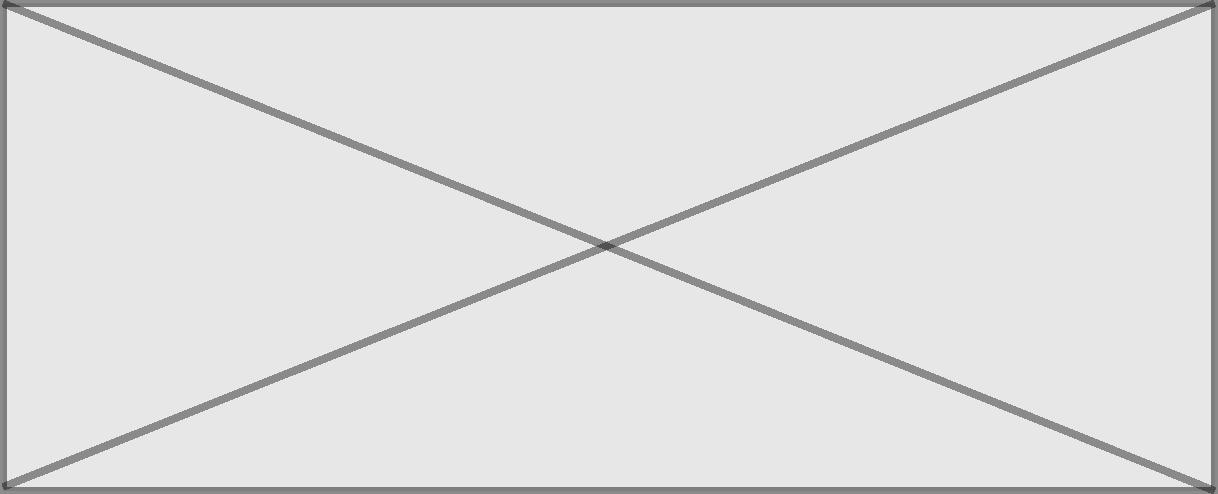
\includegraphics[width=0.7\textwidth]{placeholder.pdf}
  \caption{%
    Evolution and milestones set by the \gerda\ experiment through its three experimental
    phases. The background index, the exposure gain, the neutrinoless double-beta decay
    half-life sensitivities and upper limits are tracked in time.
  }
\end{figure}

The \phasetwop\ upgrade is partly also a test bench for the next-generation successor of
\gerda\ in the field of double-beta decay physics with \gesix, the LEGEND experiment. The
collaboration, formed in October 2016 from the \gerda\ and \majorana~\cite{Abgrall2014}
(the latter experiment searching for \onbb\ with germanium detectors in \fillme, USA),
pursues the goal of building a tonne-scale \gesix\ experiment and reaching the
$\mathcal{O}(10^{27})$ sensitivity scale. The first phase of the experiment, LEGEND-200,
deploys 200~kg of germanium in the existing \gerda\ infrastructure at LNGS and it is
currently in commissioning phase. LEGEND-1000 \fillme.

As the present thesis work focuses on \gerda\ \phasetwo\ data, the description of the
experimental setup and the main analysis techniques given in the following will be limited
to that time period. The chapter is structured as follows. In
\cref{sec:gerda:setup} a general overview of the apparatus is given \fillme.

\section{Overview of the experimental setup}\label{sec:gerda:setup}

The \gerda\ experiment is located in hall~A of the LNGS laboratories, at a depth of about
3500~m water equivalent, to suppress cosmogenically-induced background sources. The
germanium detectors are arranged into strings within a cryostat filled with 64~m$^3$ of
liquid argon (LAr), which acts as a shielding and cooling medium at the same time. The
cryostat itself is enclosed by a large tank containing 590 m$^3$ of ultra-pure water.
Besides the additional shielding effect, this water layer act as a medium for a
\v{C}erenkov veto system with 66 photomultiplier tubes (PMTs) against muons. An array of
scintillating panels is installed on the top of the clean room to complete the muon veto
system~\cite{Freund2016}. A simplified representation of the experimental setup is given
in \cref{fig:setup:artistview}.

\begin{figure}
  \centering
  \begin{tikzpicture}[fill=white]
    \node at (0,0) {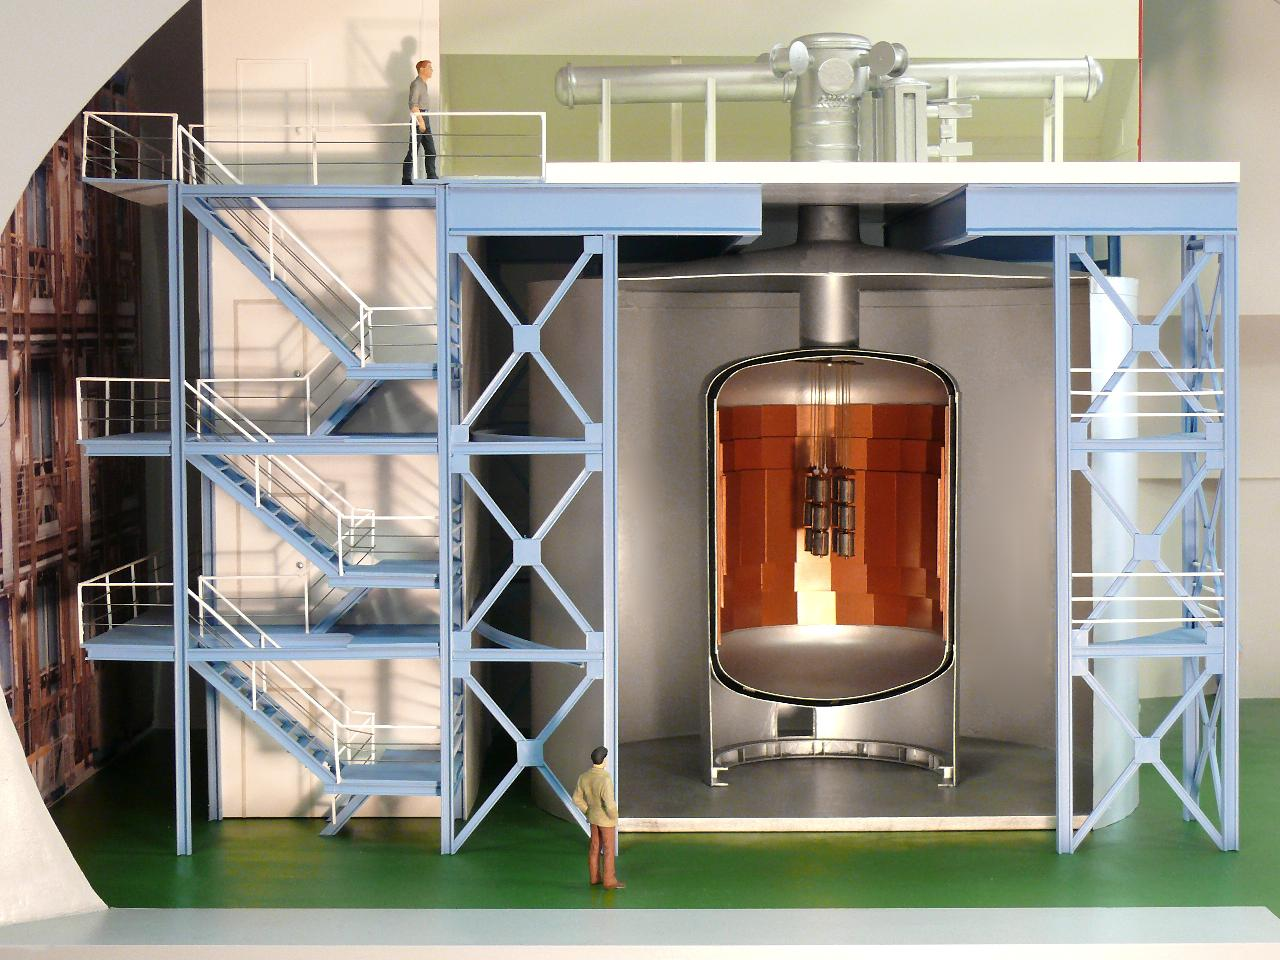
\includegraphics[height=7cm]{setup/gerda-artist.jpg}};
    \node(e) at (3.5,3.3) [rectangle,draw,fill] {\textsc{muon veto}};
    \draw[thick,red,->] (e.south) .. controls +(0,-1) and +(0,1) .. (2.3,2.4);
    \node(a) at (1.6,-1.2) [rectangle,draw,fill] {LAr};
    \node(b) at (3.2,1.6) [rectangle,draw,fill] {\gesix\ \textsc{detectors}};
    \draw[thick,red,->] (b.south) .. controls +(0,0) and +(1,0) .. (1.9,-0.4);
    \node(c) at (-1.5,1.6) [rectangle,draw,fill] {H$_2$O};
    \draw[thick,red,->] (c.south) .. controls +(0,0) and +(-1,0) .. (0,-1);
    \node(d) at (0,3) [rectangle,draw,fill] {Cu \textsc{shielding}};
    \draw[thick,red,->] (d.south) .. controls +(0,0) and +(-1,0) .. (1,0);
    \node at (-1.5,-3.15) [rectangle,draw,fill] {\small Laboratori Nazionali del Gran Sasso (LNGS)};
  \end{tikzpicture}
  \caption{%
    Artist view of the \gerda\ experimental setup. The experiment, installed in hall A of
    the Gran Sasso National Laboratories in Italy, deploys an array of germanium detectors
    enriched in \gesix\ bare in liquid argon, together with a liquid argon scintillation
    light veto system. The cryostat is submerged in a water tank to provide additional
    shielding from external background sources. A muon veto plastic scintillating panel
    system is installed on the top of the whole structure.
  }\label{fig:setup:artistview}
\end{figure}

\marginnote{Detectors}
The \gerda\ \phasetwo\ array is organized in 7 vertical strings, holding 40 detectors in
total. The detectors can be divided in three groups: the BEGe detectors, the semi-coaxial
\m{ANG} and \m{RG}, and the semi-coaxial \m{GTF} detectors. The detectors of the first two
groups are made of germanium enriched in \gesix, the third group includes detectors with
natural isotopic germanium abundance.

All \gerda\ HPGe detectors are made of high-purity p-type germanium, which is initially
used to pull crystals, typically fuse-shaped (see fig.~4.1a in \cite{Yonenaga2019}).
Crystals are then cut in slices, and each of them is further processed according to the
final detector geometry. The electrodes for signal read-out and voltage biasing are then
fabricated on the detector surface. The n+ contact, where the external voltage is applied,
wraps around the detector. It is obtained by deposition of a lithium layer on the surface,
which diffuses below the surface until a depth of $\sim$1~mm during the subsequent thermal
annealing cycles. The presence of lithium impurities effectively creates a region with
decreased charge collection efficiency (CCE), or `dead-layer' even when biased at
full-depletion voltages.  In this region, the CCE is zero at the surface and reaches its
maximal value at the full charge collection depth (FCCD). The p+ electrode, where the
signal is read out, is instead fabricated by boron implantation, and the dead layer it
produces is typically smaller, at the level of hundreds of microns. The two conductive
surfaces are separated by an insulating region, which is typically produced by excavating
a `groove'. In some cases such groove is passivated by deposition of a oxide \fillme\
layer.

The \gerda\ \phasetwo\ detectors can be classified according to two different geometry
types: semi-coaxial and BEGe. In the semi-coaxial design, a bore-hole is excavated along
the central axis to accomodate the p+ electrode. With such a configuration, relatively
large detector masses can be achieved, of the order of 2--3~kg. The \ANG{} (5), \RG{} (2)
and \GTF{} (3) detectors, inherited from the \hdm\ and \igex\ experiments and already used
in \phaseone, are of the semi-coaxial type. Their total mass amounts to 23.2~kg of
germanium.  For \phasetwo, 20~kg of enriched germanium was procured by the \gerda\
collaboration for the production of 30 new diodes of the BEGe type. The Broad Energy
Germanium detector design does not include a bore-hole, therefore the p+ contact is a
small, dot-shaped surface at the center of one of the two detector sides. The absence of a
bore-hole makes this kind of detectors harder to full deplete, requiring lower impurity
concentrations and smaller masses, generally lower than 1~kg. A detailed description of
the characteristics of the BEGe detectors, from germanium procurement to diode production
can be found in~\cite{Agostini2015e, Agostini2018a, Agostini2019}.

\marginnote{Array}
As already mentioned, the \gerda\ \phasetwo\ detectors are arranged into 7 strings, packed
closely together as depicted in \cref{fig:setup:magevolumes}a. The detector holder unit
consists of and intrinsically radio-pure silicon plate and vertical copper bars to connect
the units between themselves within a string. See fig \fillme

\marginnote{LAr veto}
To improve the sensitivity on the \onbb\ half-life and enter the \bkgfree\ regime, an
additional active veto system to collect the LAr scintillation light produced by
background events was designed and installed during the upgrade works for \phasetwo. A
cylindrical hybrid design was chosen to detect the light information: a curtain made of
light-guiding plastic fibers coupled to a ring of silicon photomultipliers (SiPMs) to
surround the array and PMTs on the top (9) and on the bottom (7) (see
\cref{fig:setup:magevolumes}f). To enhance the light collection efficiency two copper
shrouds (visible in \cref{fig:setup:magevolumes}e) coated with a reflective \tetratex\
layer were added between the fiber shroud and the PMT holder plates. The latter were
coated with a reflective VM2000 layer. Another light collection improvement introduced by
the \phasetwo\ upgrade is the installation of nylon (mini-)shrouds enclosing each detector
string (\cref{fig:setup:magevolumes}d). The presence of these shrouds provides an
essential mechanical barrier to reduce the background from \kvz\ ions naturally present in
LAr, which undergo \b-decay and can mimic the \onbb\ signature at \qbb. Being made of
transparent nylon material, these shrouds, however, let the light propagate more
efficiently to a light collecting surface. To match the fibers and PMTs \fillme\ spectra
many surfaces in the close vicinity of the array were coated with tetraphenil-butadiene
(TPB), a wavelength shifting material. Coating has been applied on mini-shrouds,
fiber-shroud, copper shroud, PMTs as well as their holder plates.

\begin{figure}
  \includegraphics[height=5cm]{setup/muon-veto.jpg}%
  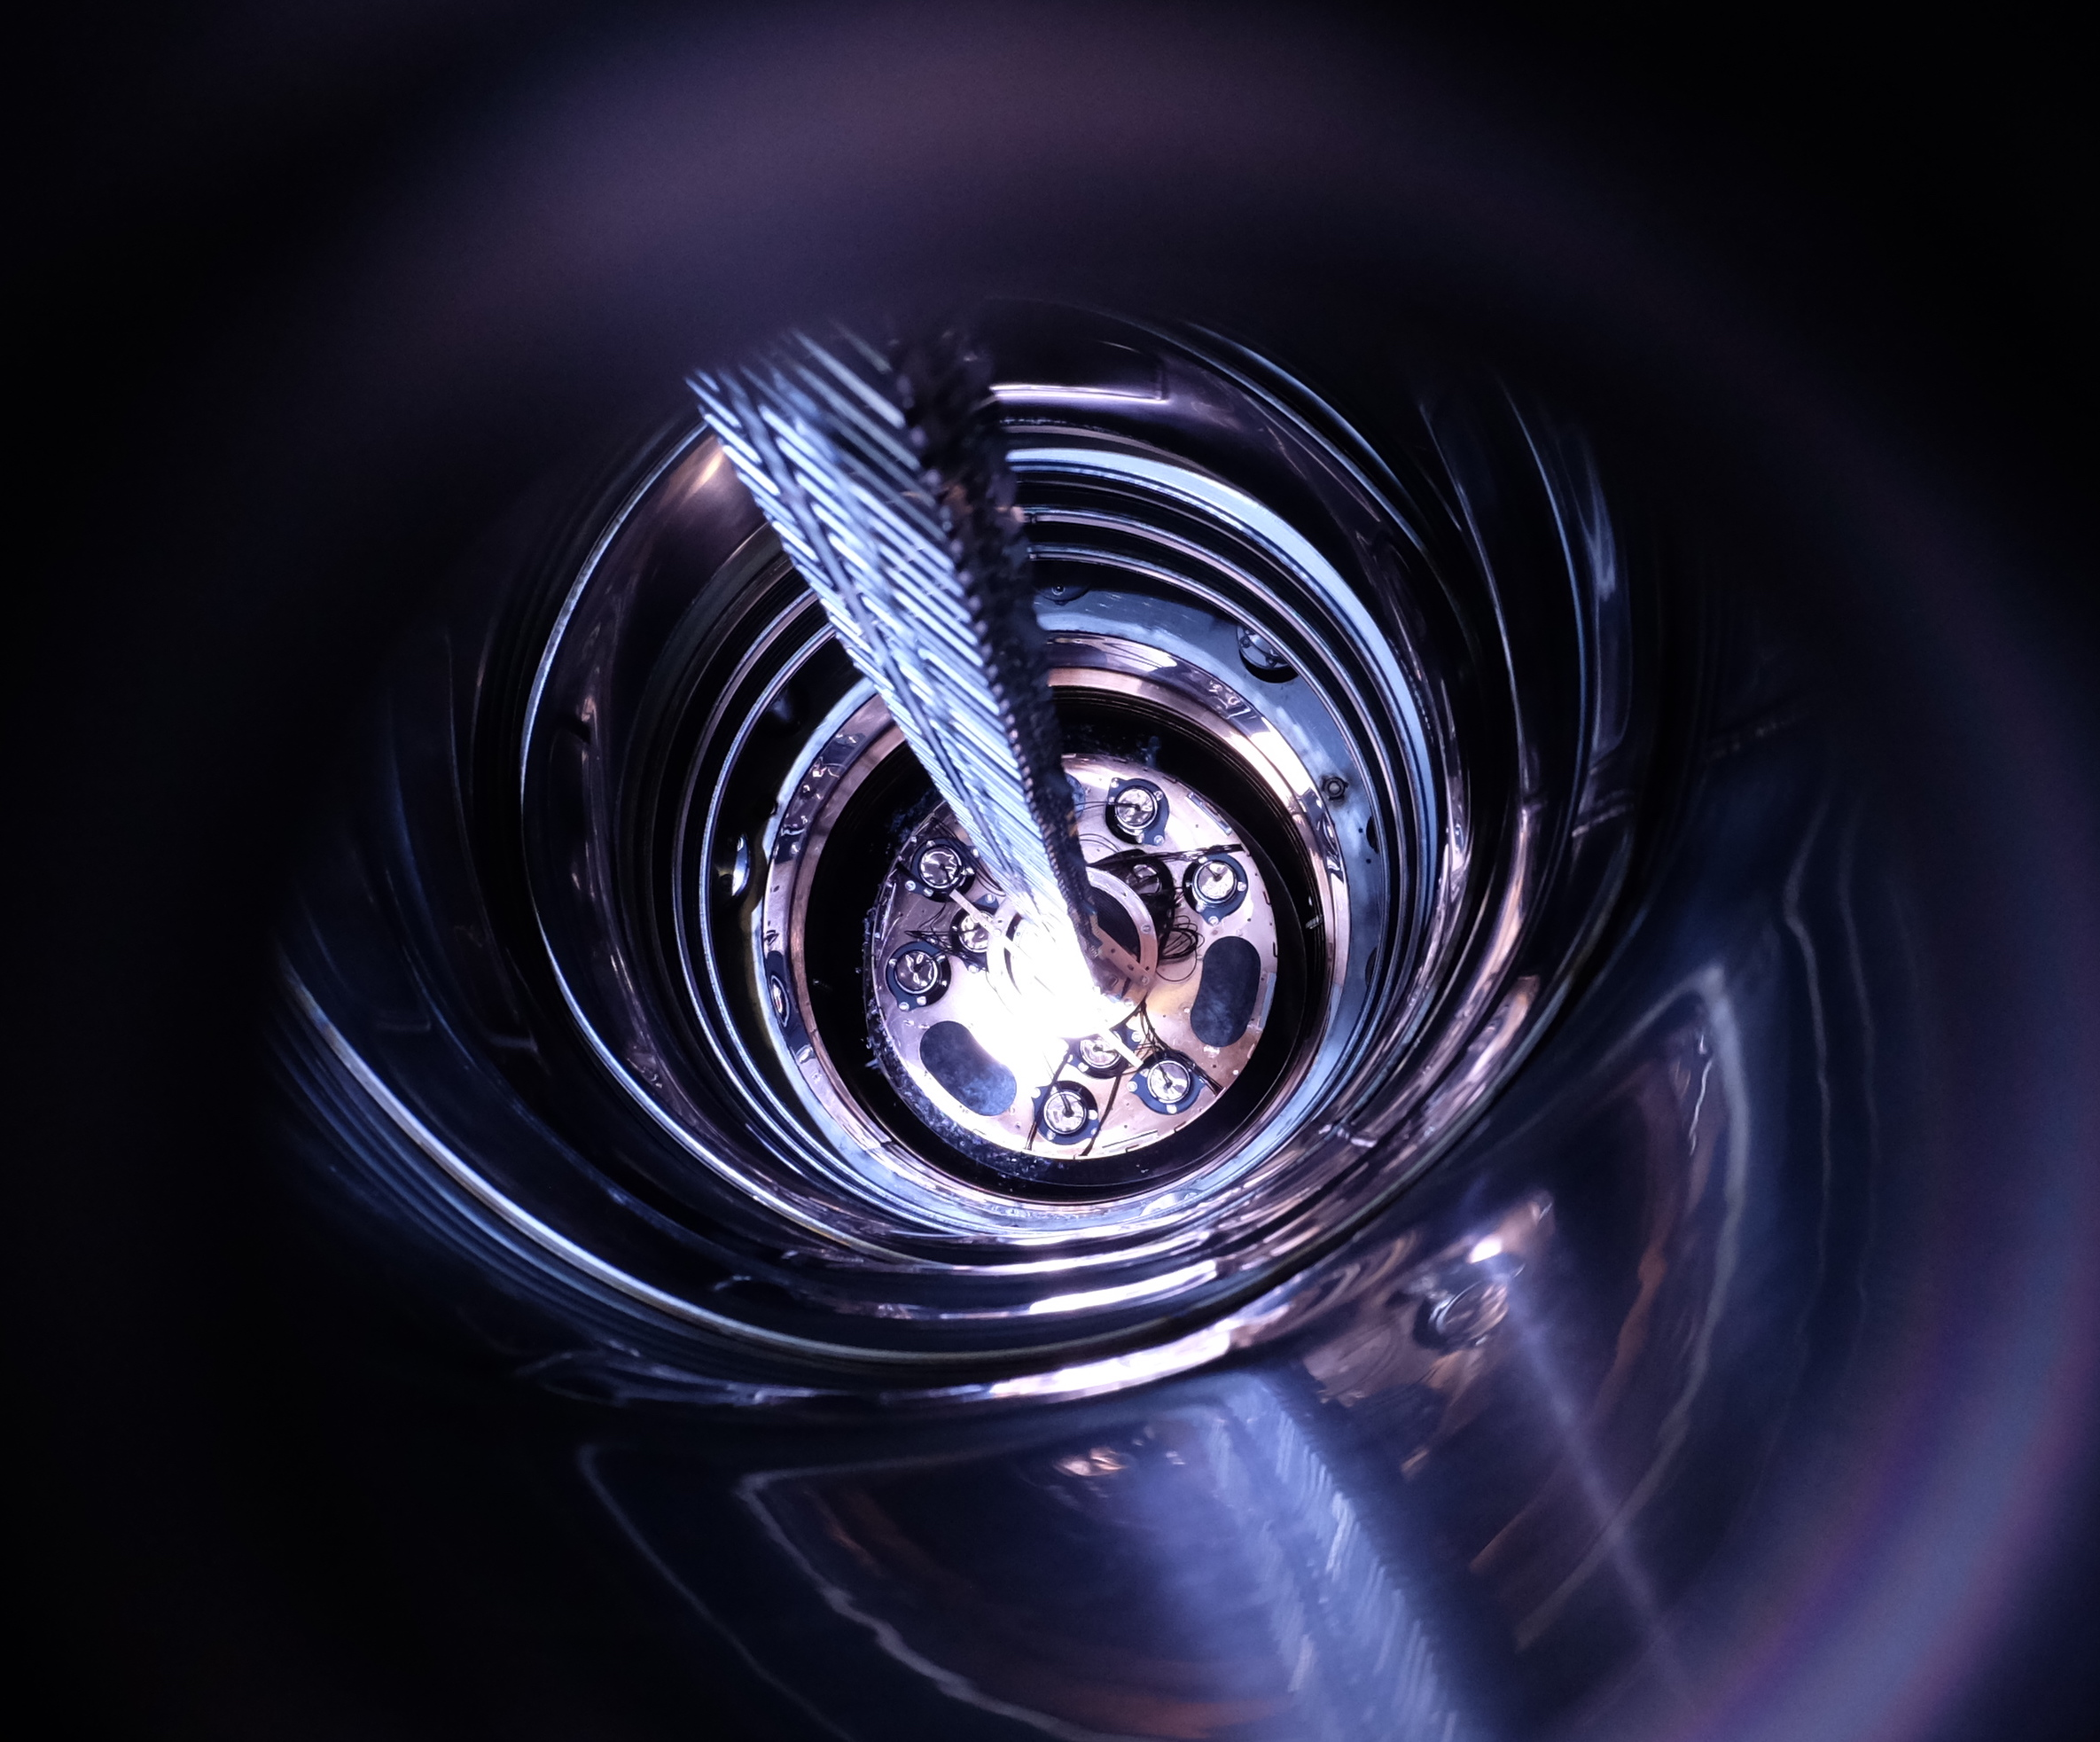
\includegraphics[height=5cm]{setup/array-lowering.jpg}\\
  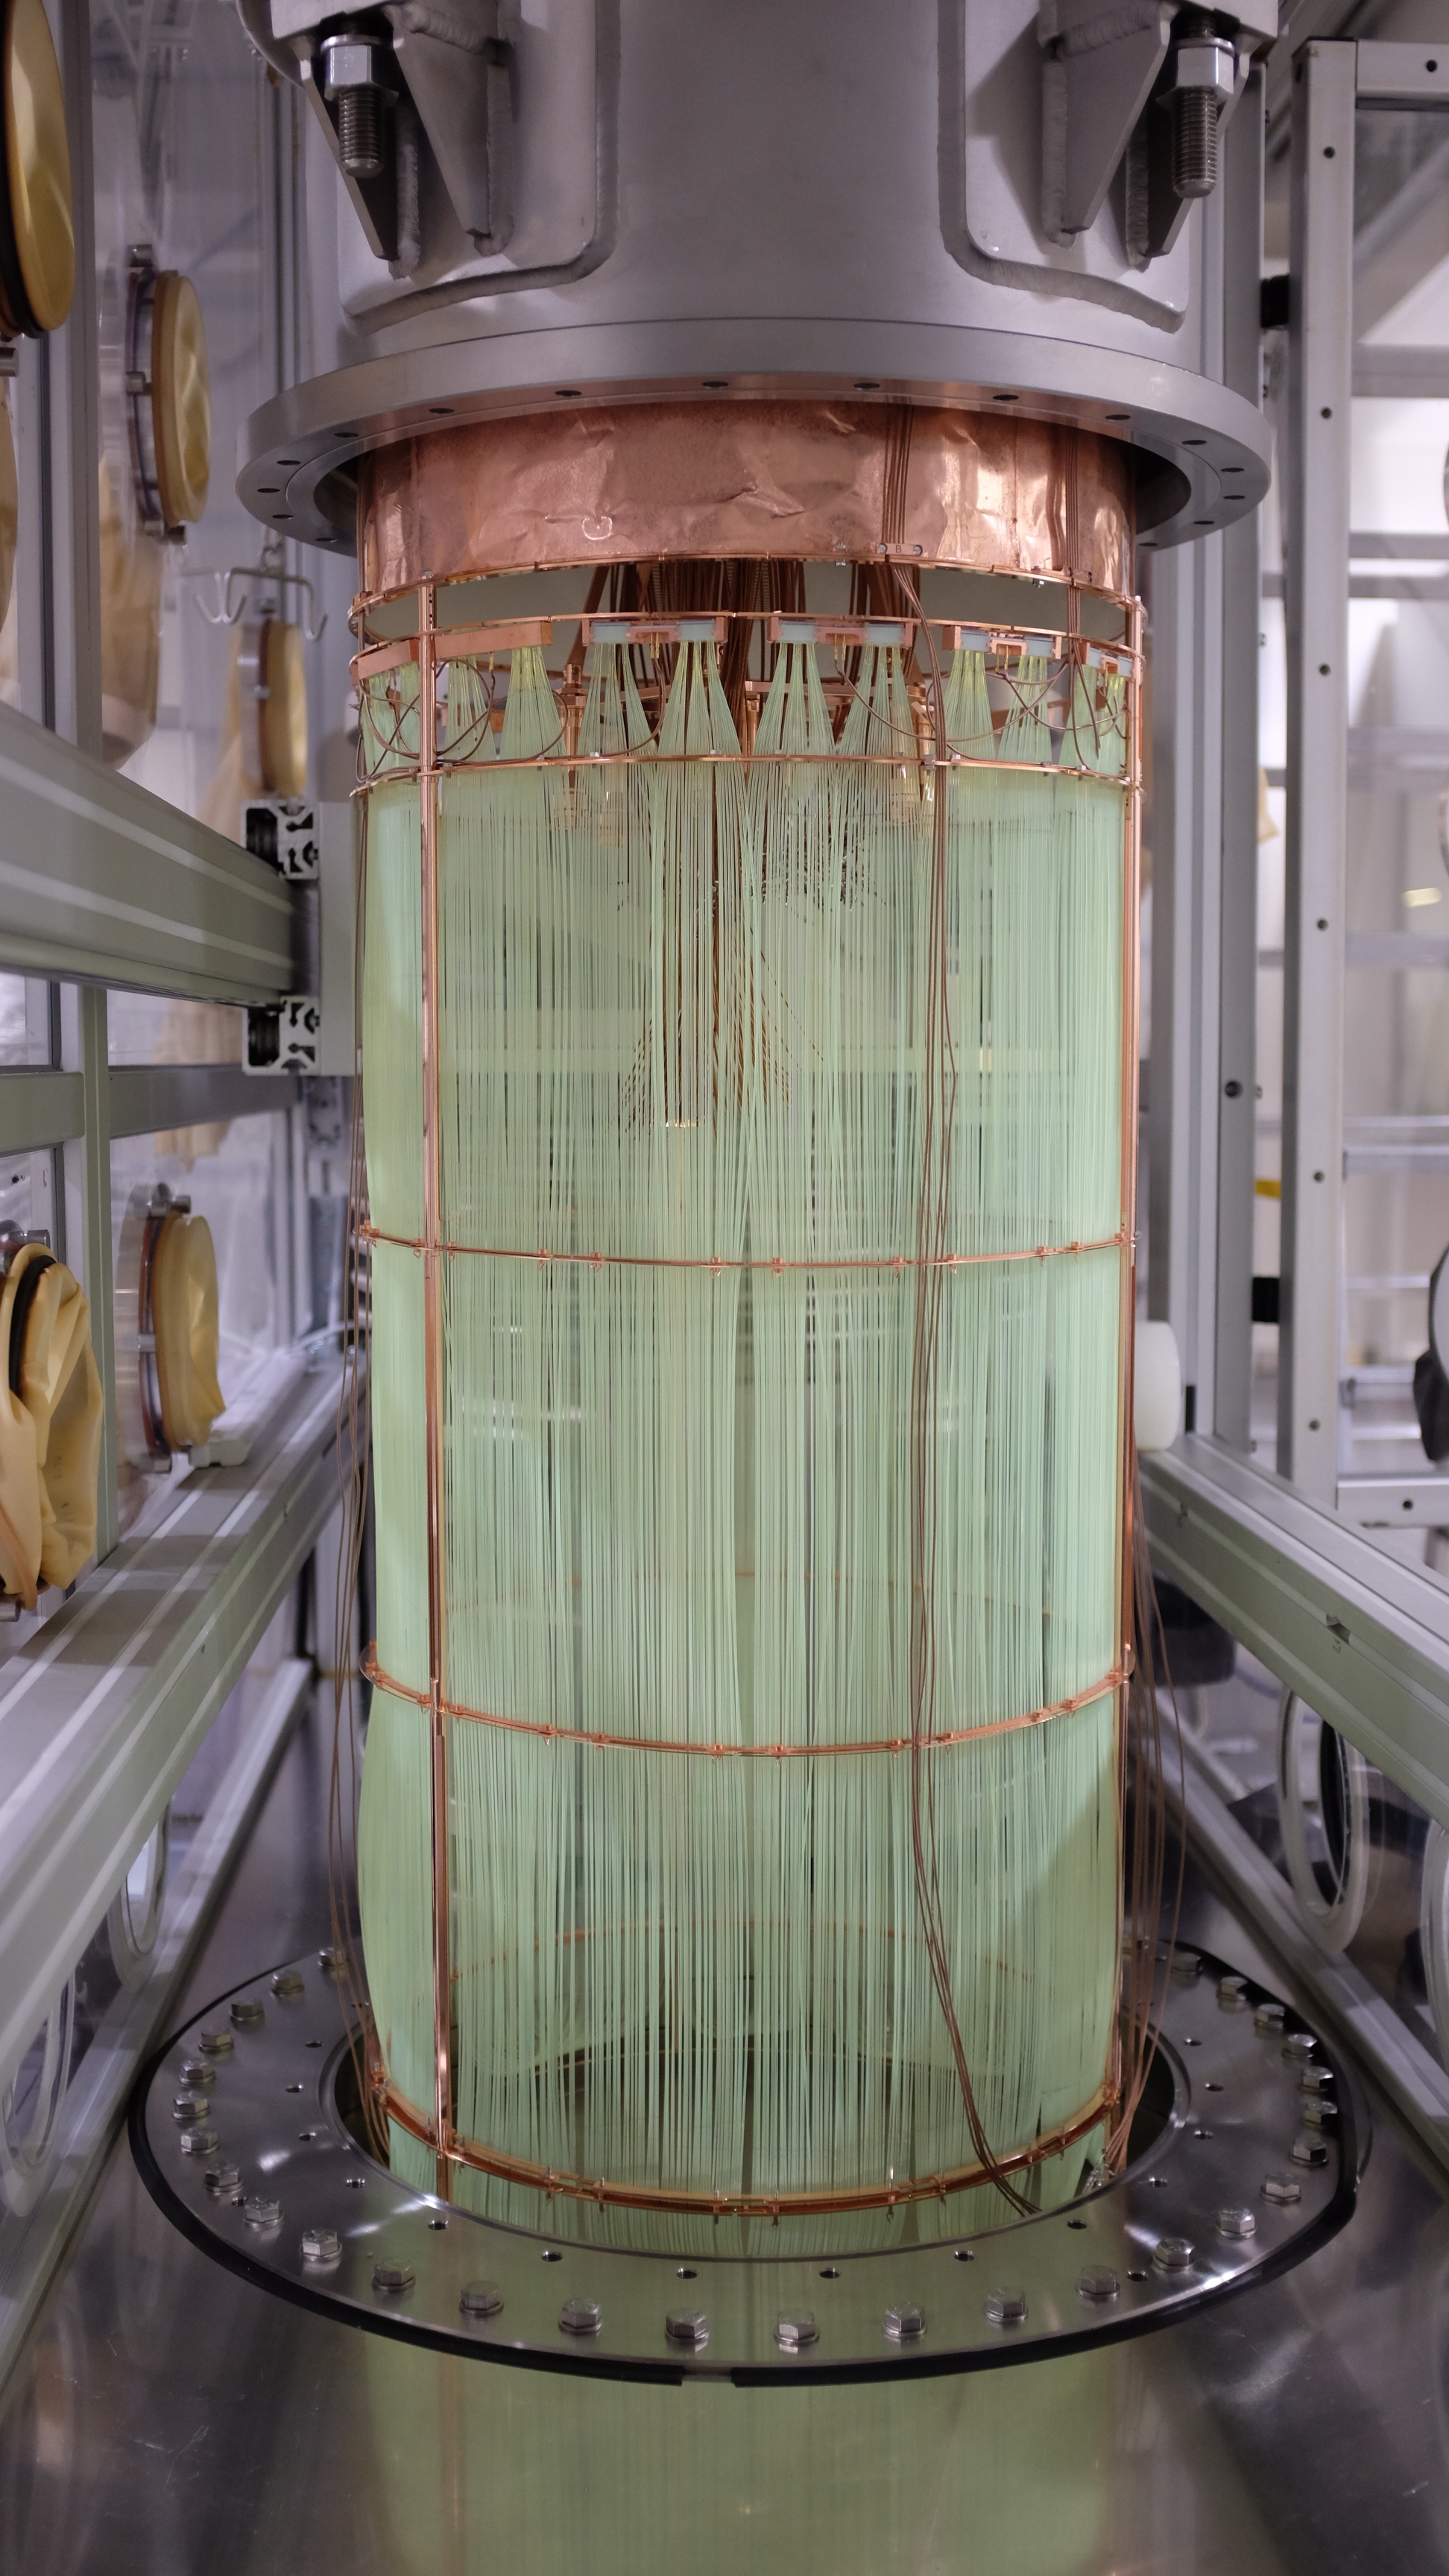
\includegraphics[height=7cm]{setup/fiber-shroud.jpg}%
  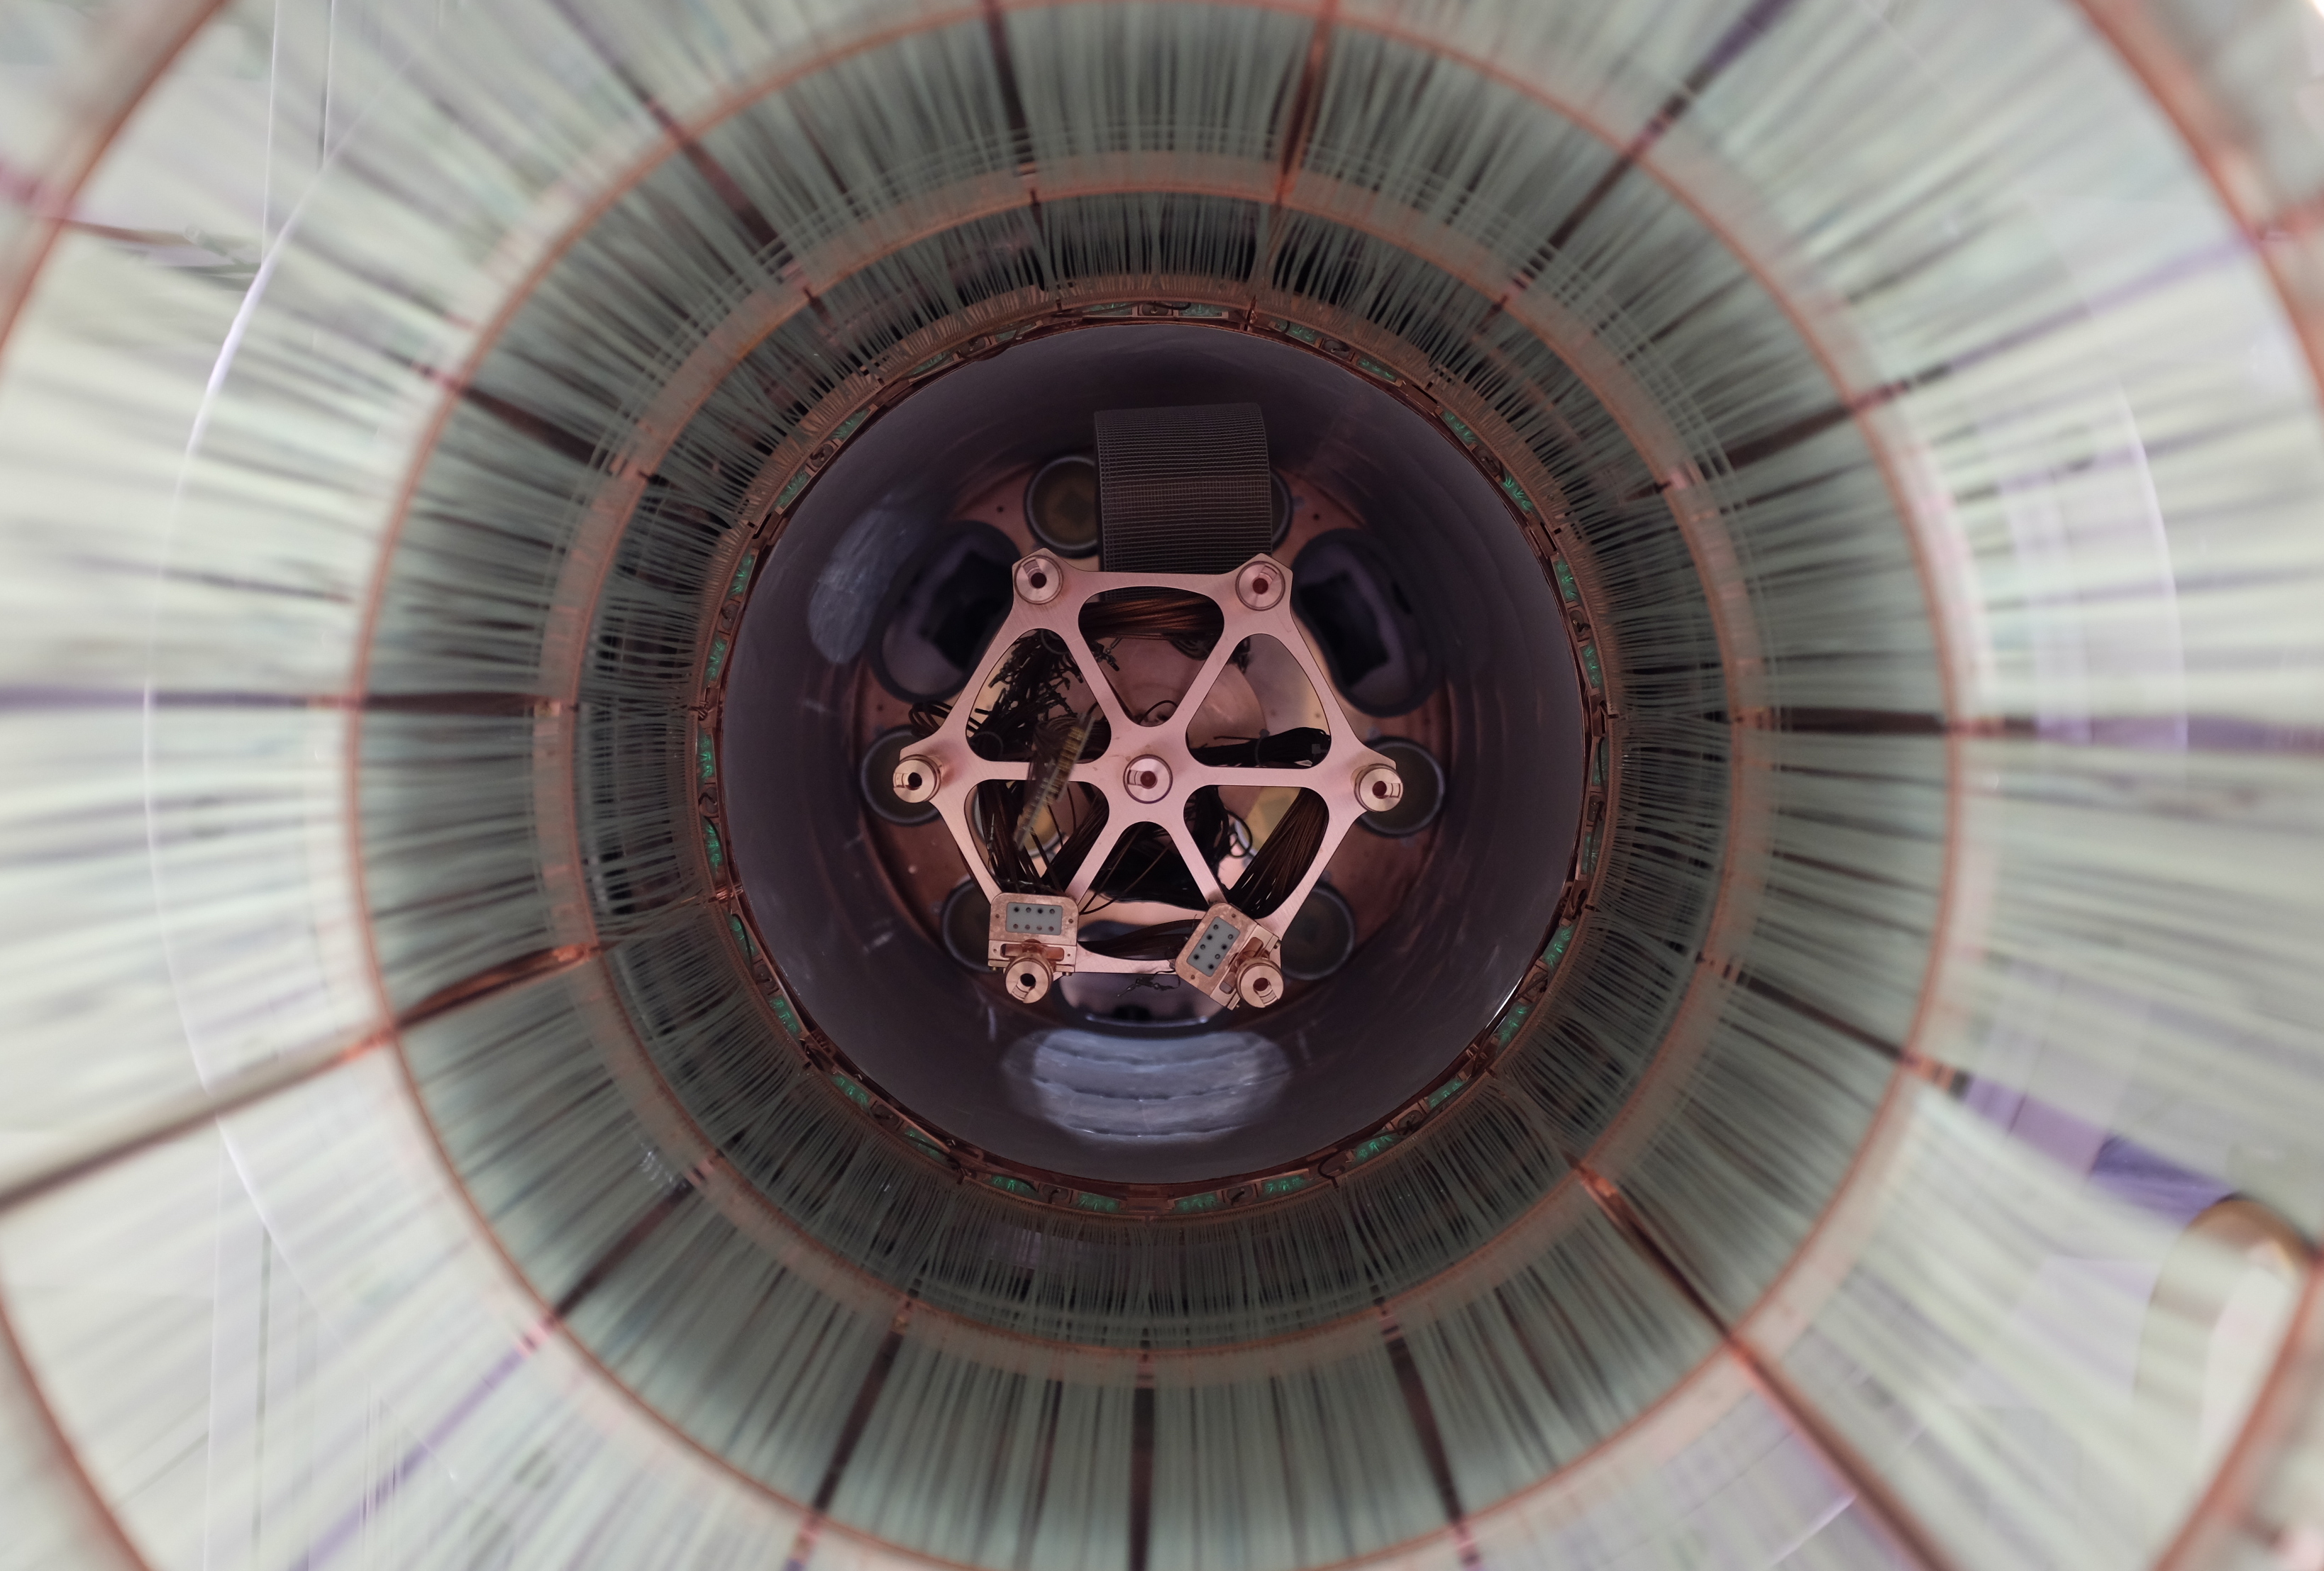
\includegraphics[height=7cm]{setup/fiber-shroud-inside.jpg}\\
  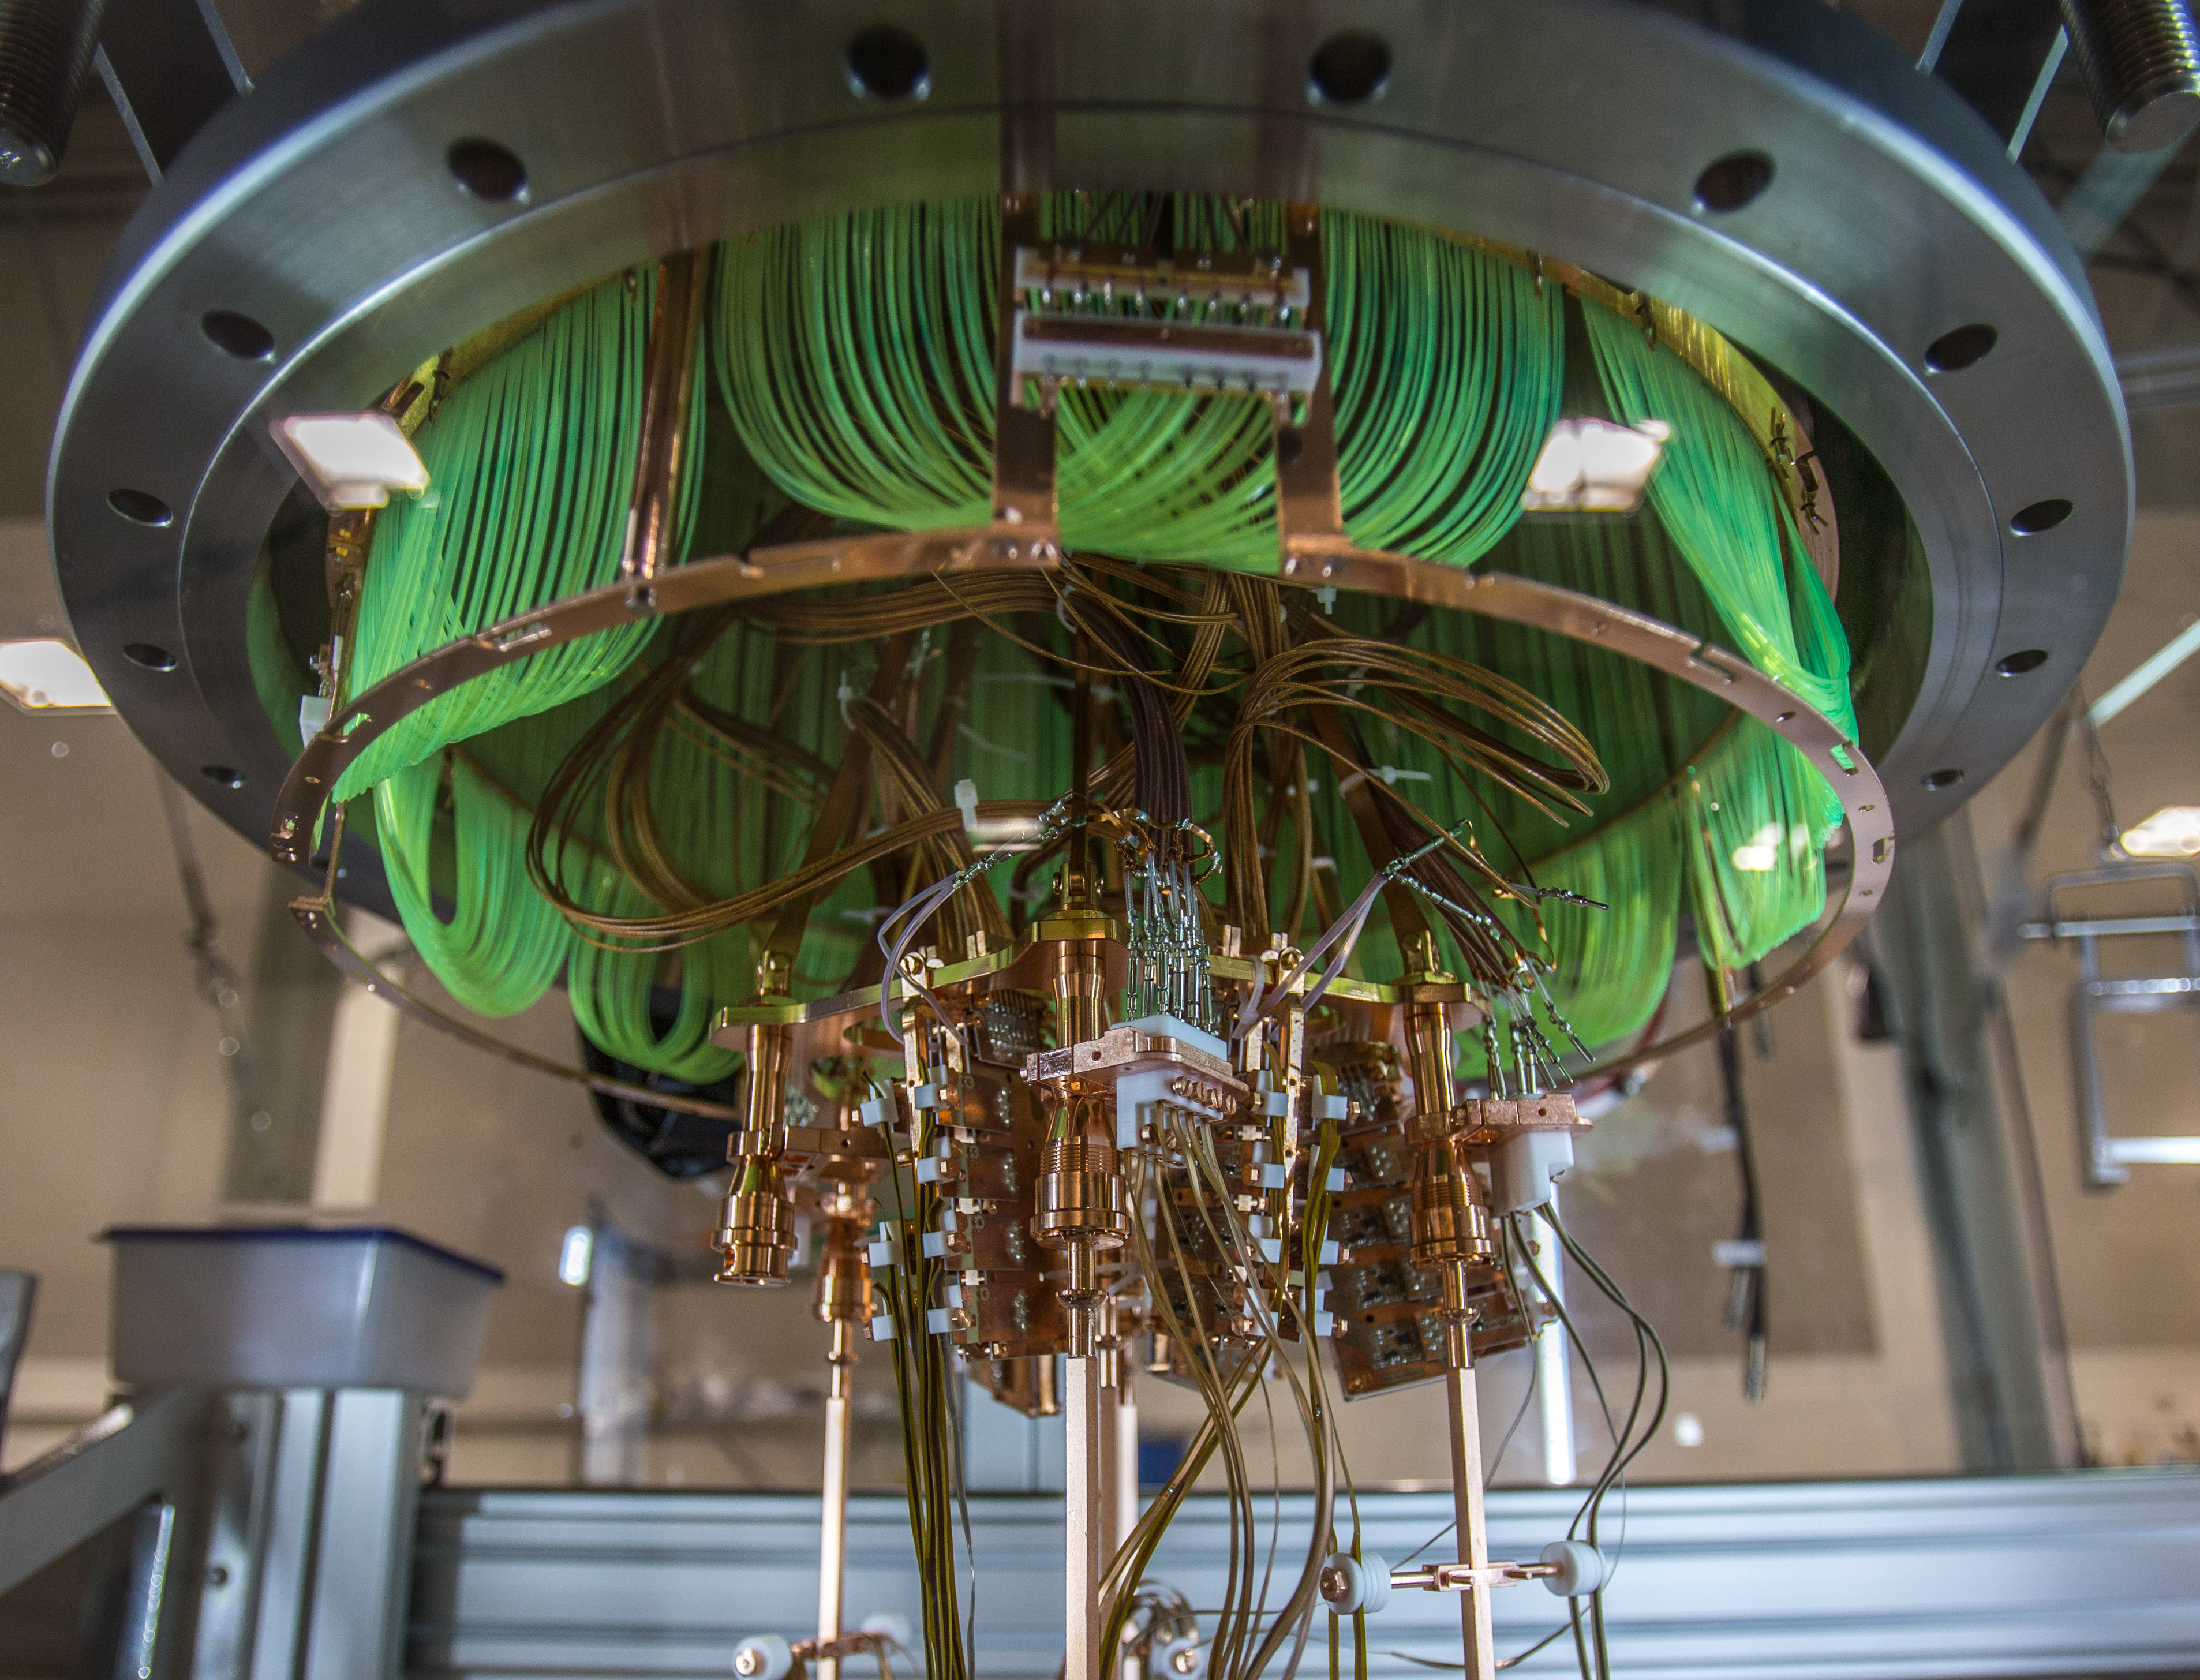
\includegraphics[height=4cm]{setup/electronics.jpg}%
  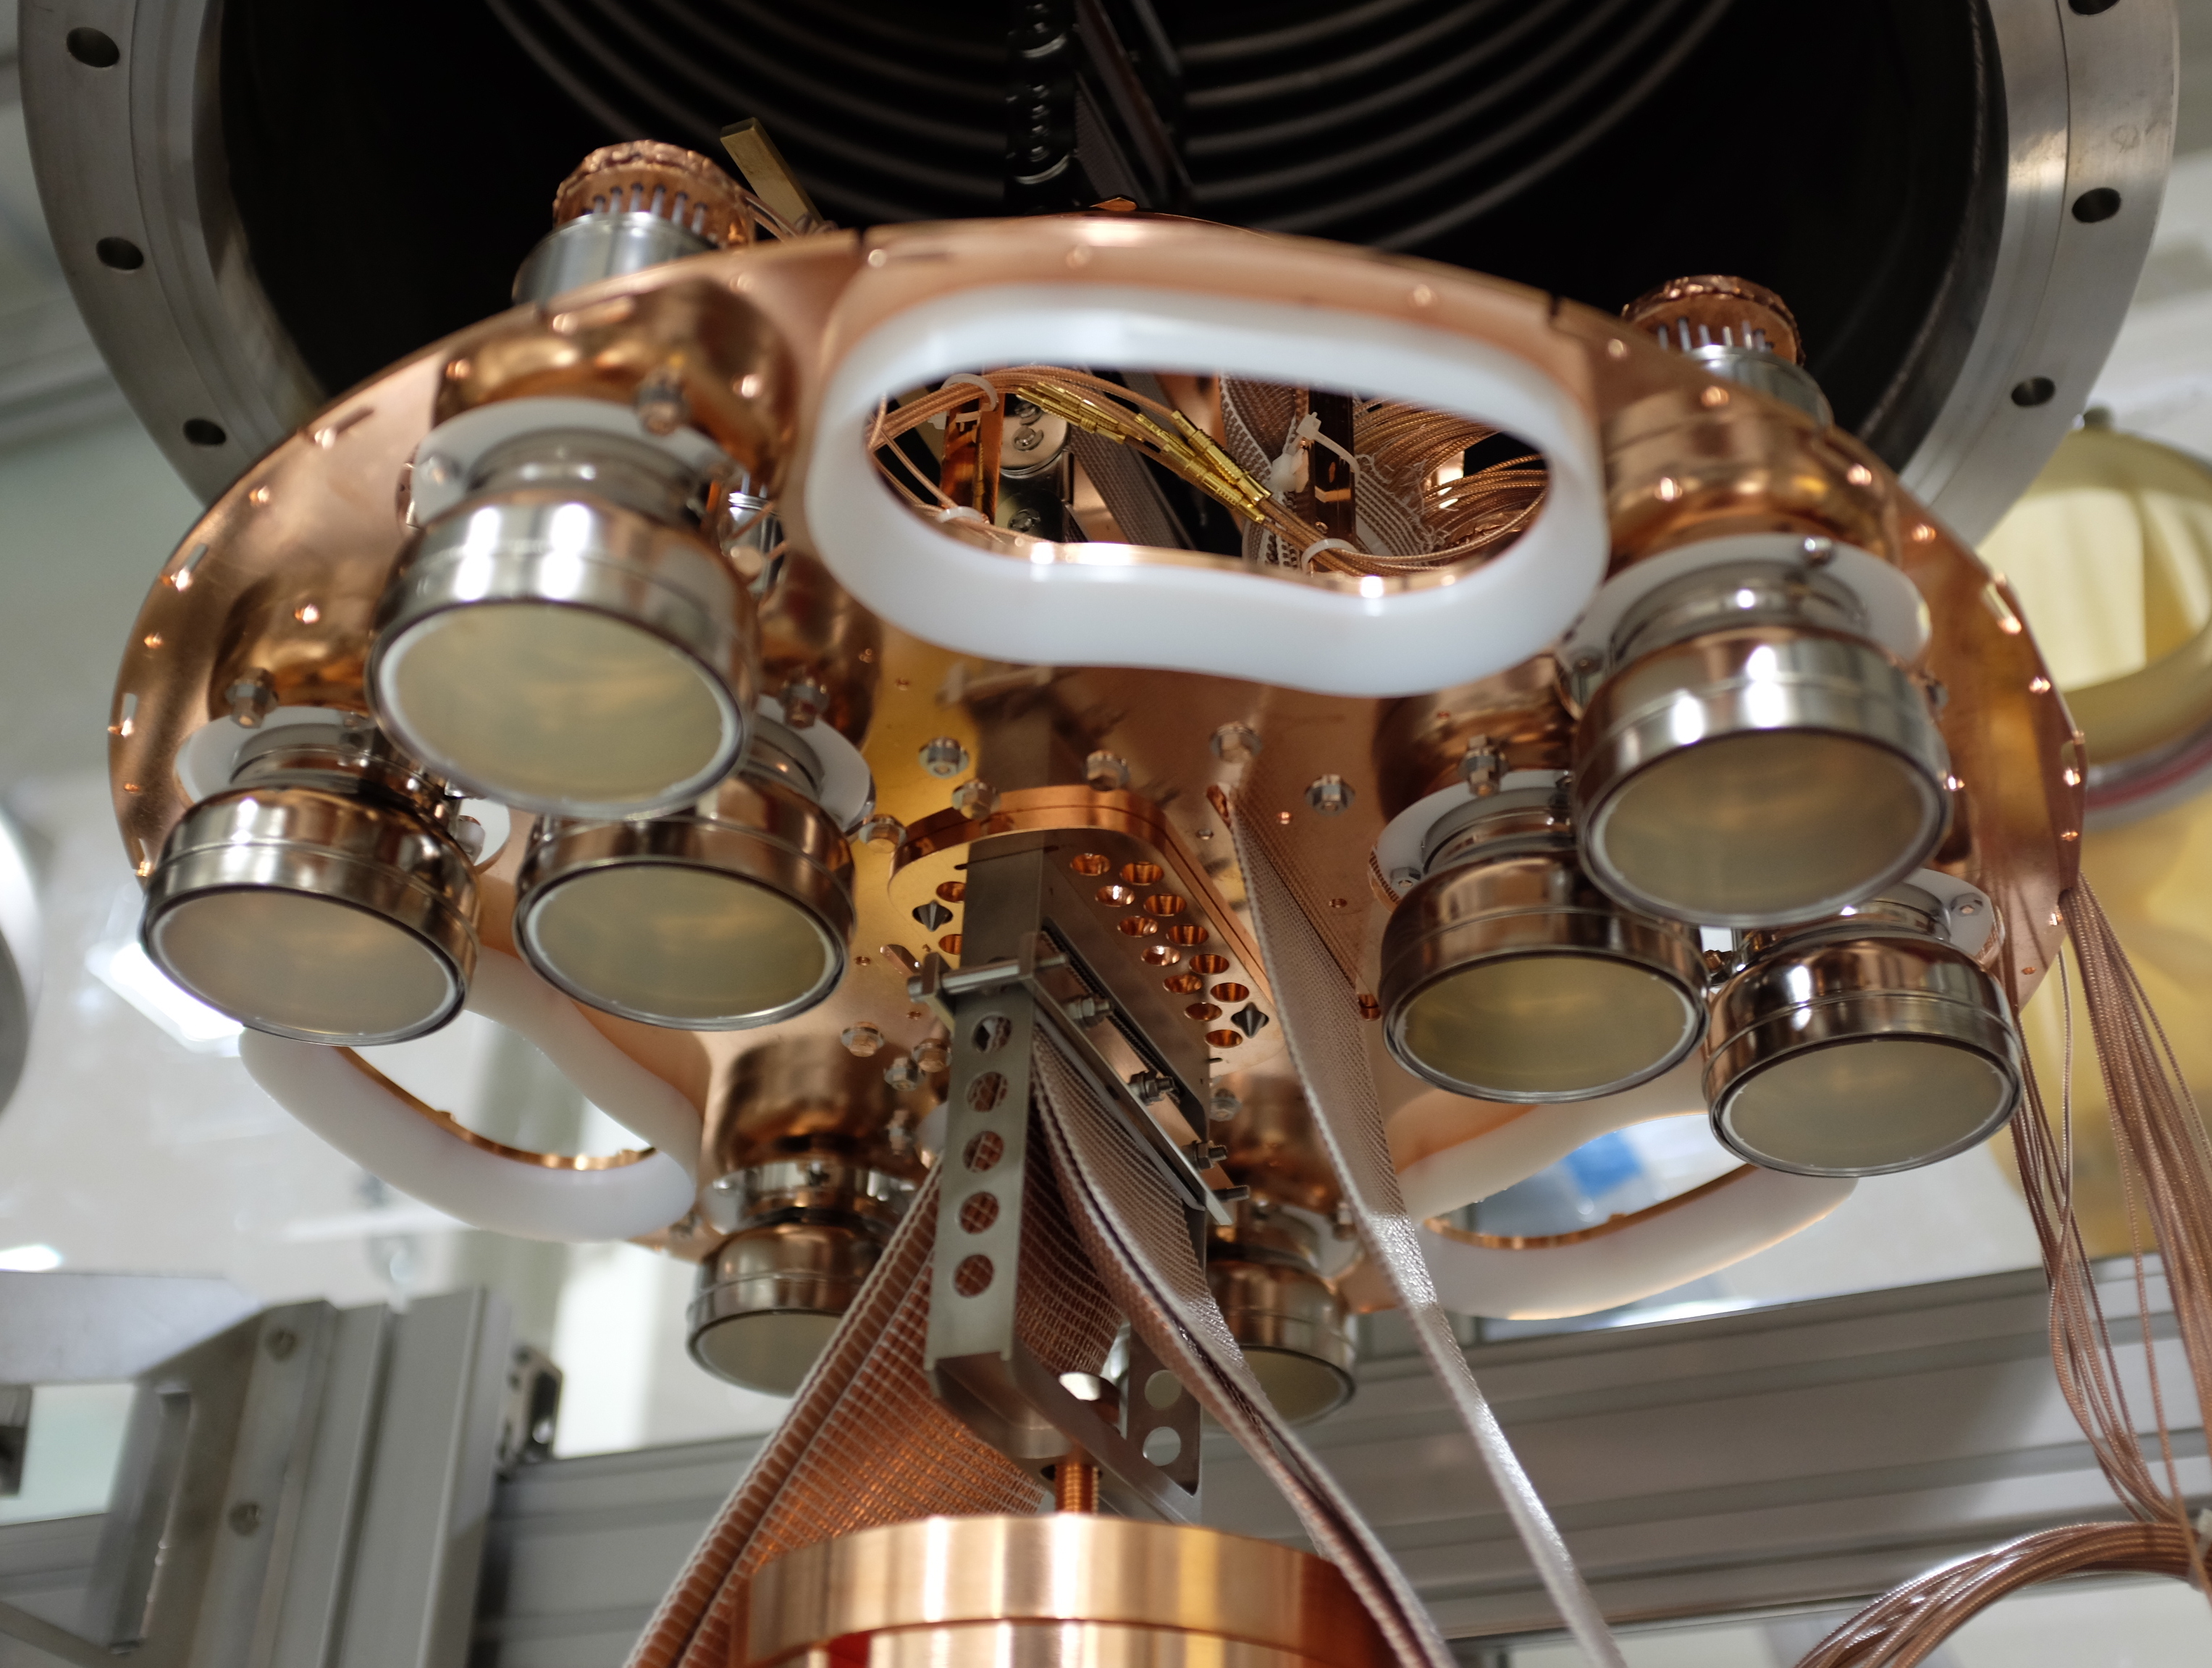
\includegraphics[height=4cm]{setup/top-pmts.jpg}%
  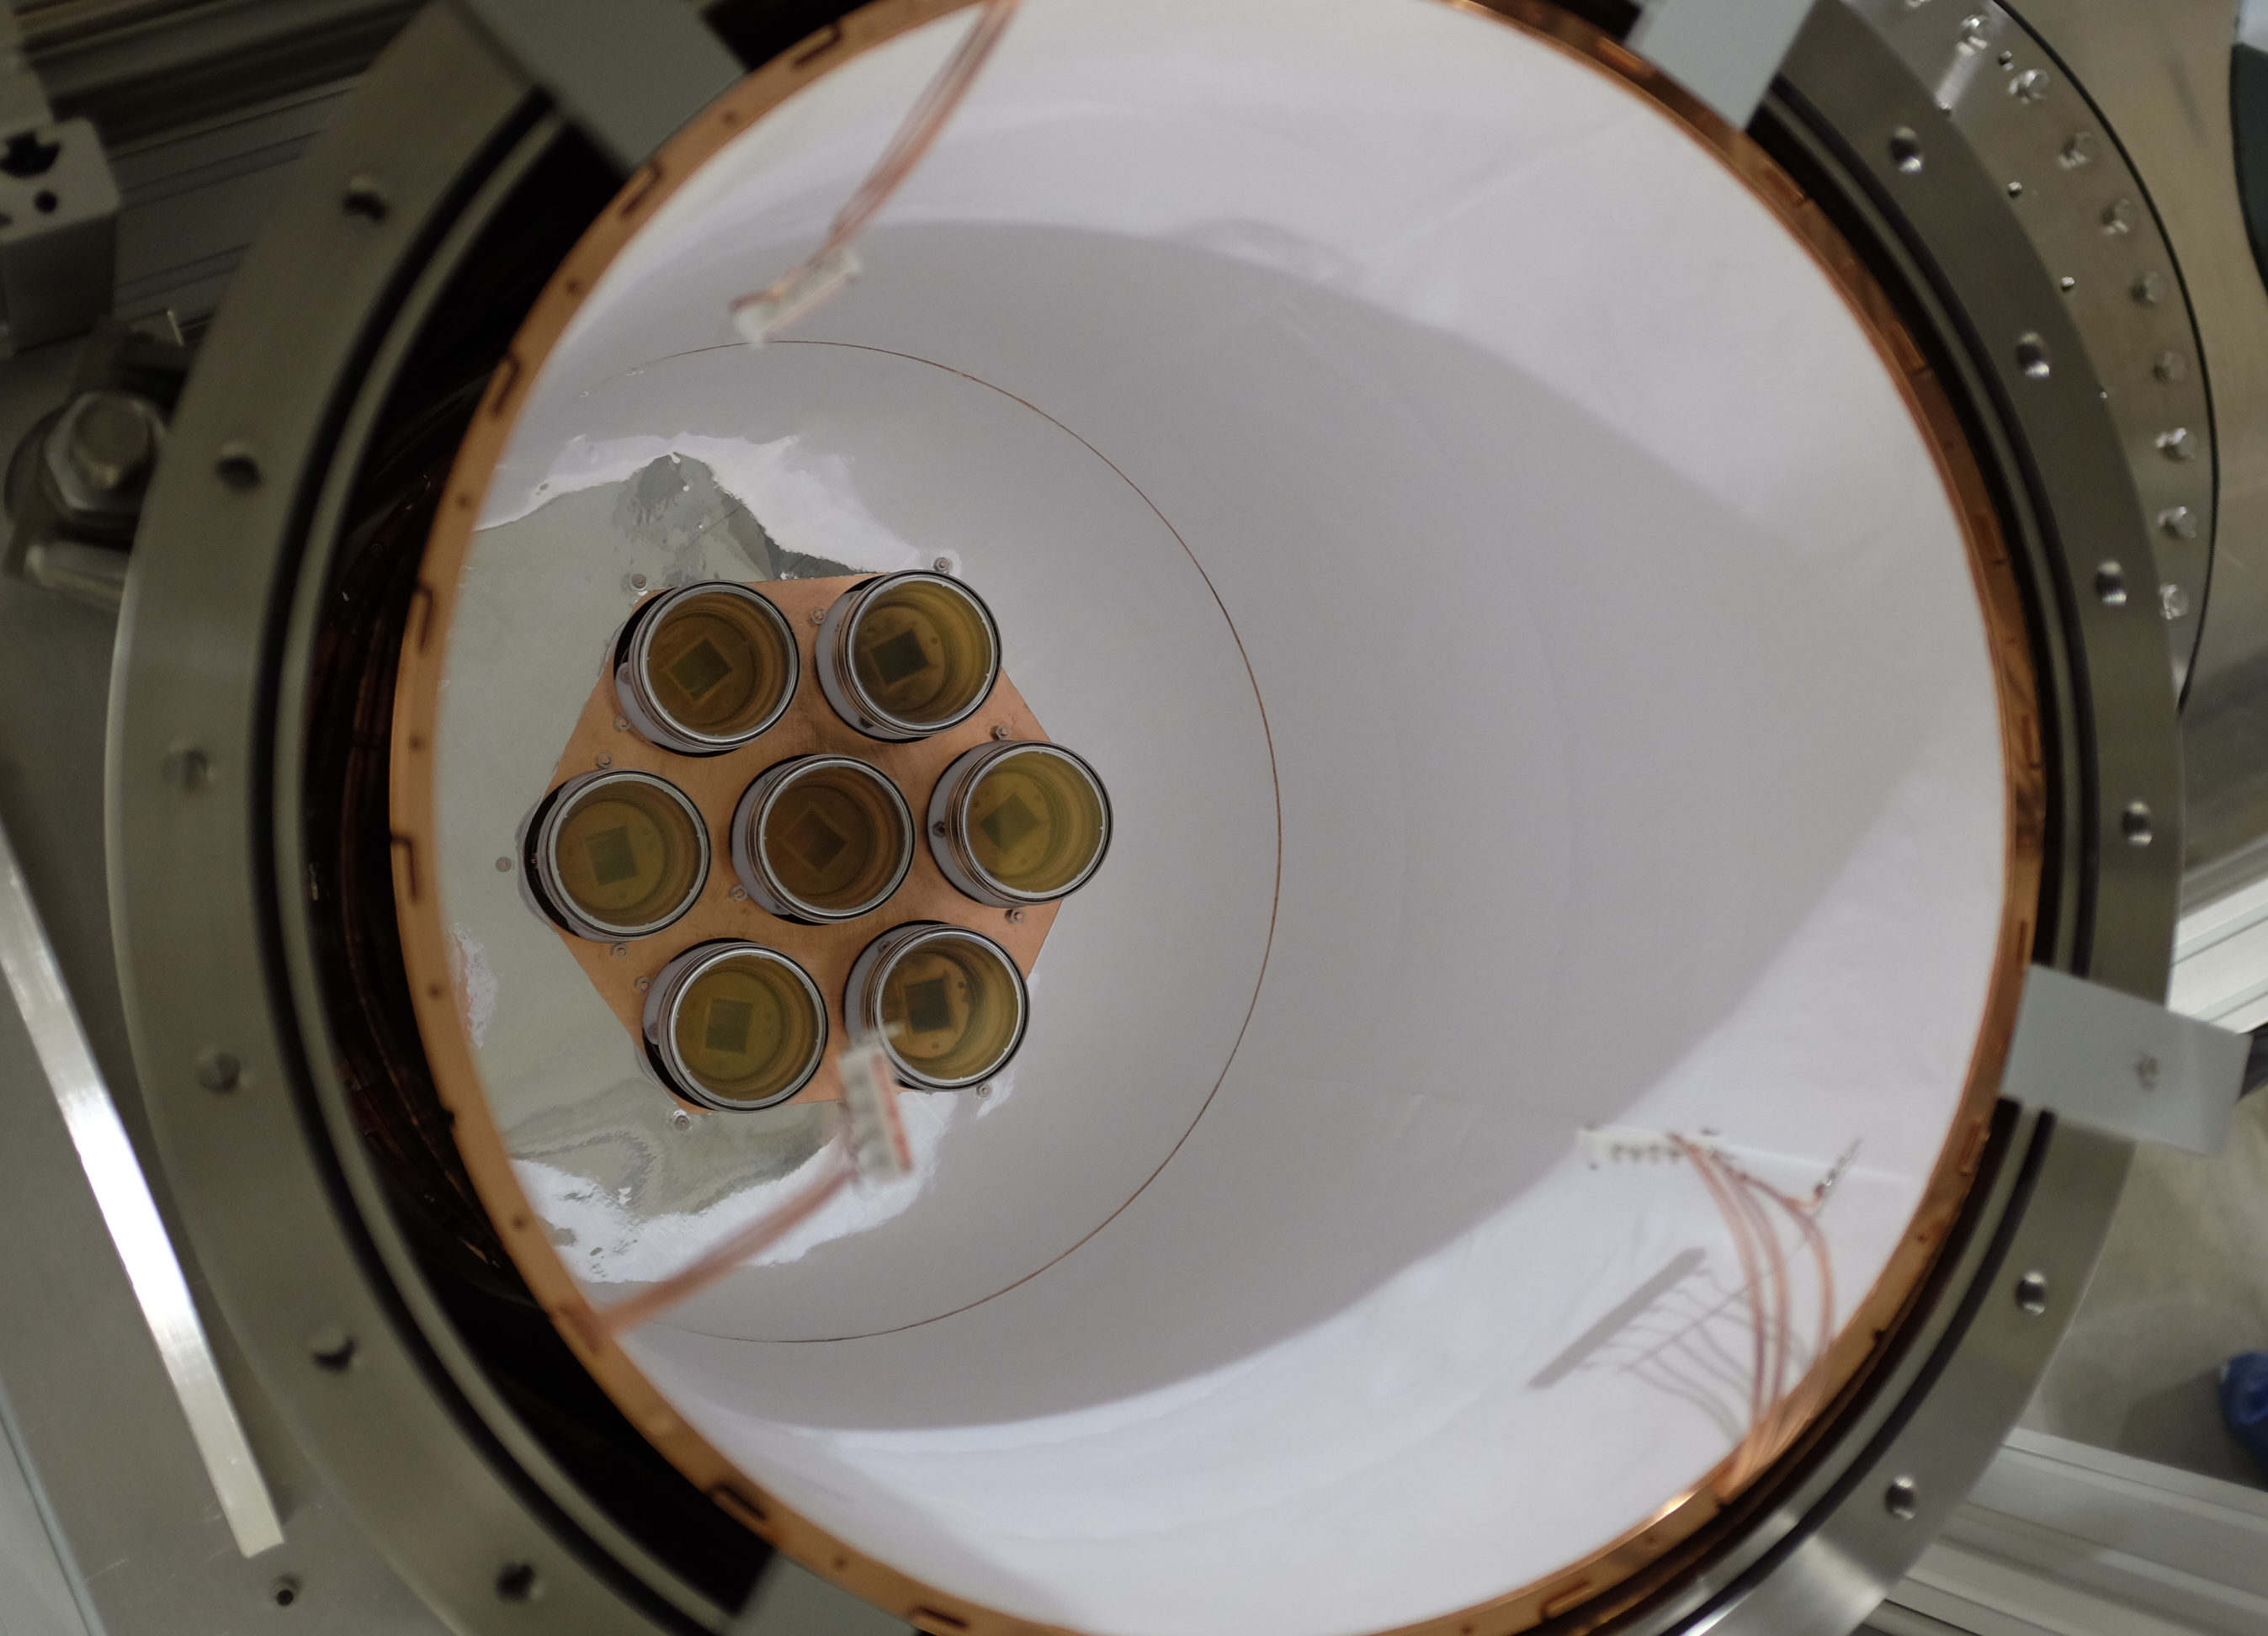
\includegraphics[height=4cm]{setup/bottom-pmts.jpg}\\
  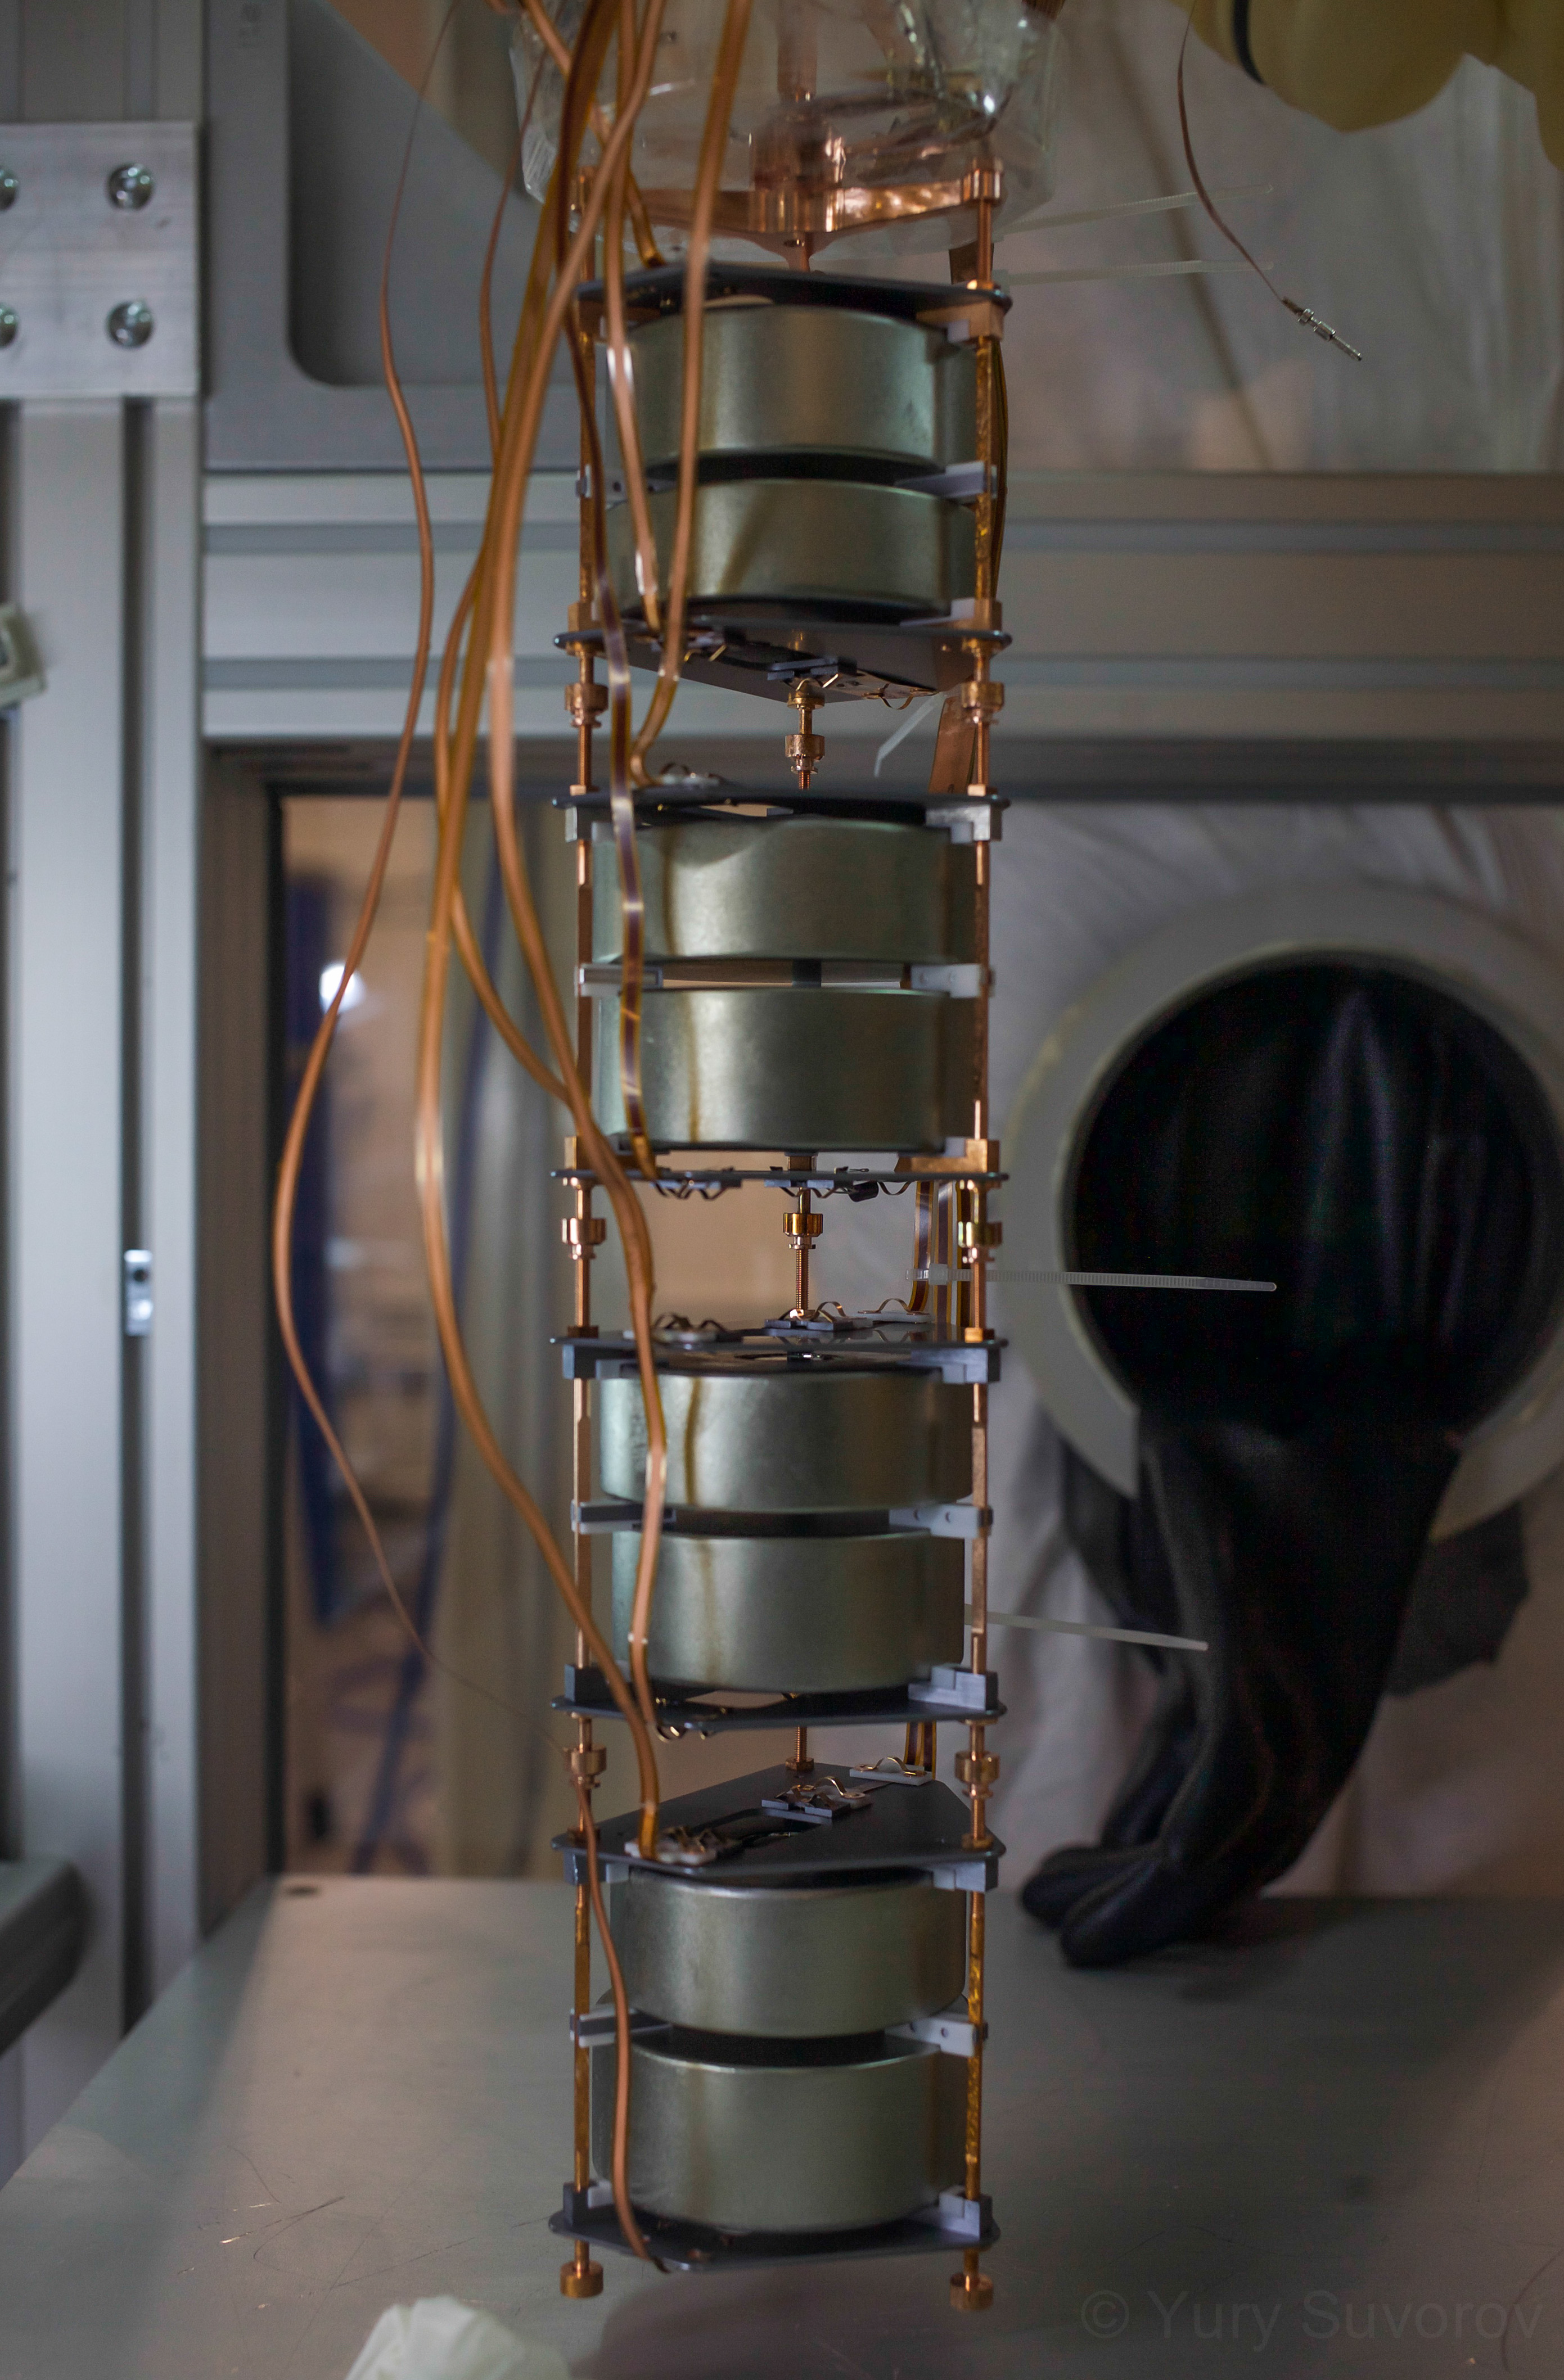
\includegraphics[height=4cm]{setup/single-string.jpg}
  \caption{%
    Various pictures of the \gerda\ \phasetwo\ setup, taken during the upgrade
    works.
  }\label{fig:setup:pictures}
\end{figure}

\marginnote{Data \\ acquisition}
A FADC system records traces from germanium detectors, PMTs and SiPMs when an energy
deposition greater than 100~keV occurs in at least one of the germanium detectors.

\begin{figure}
  \centering
  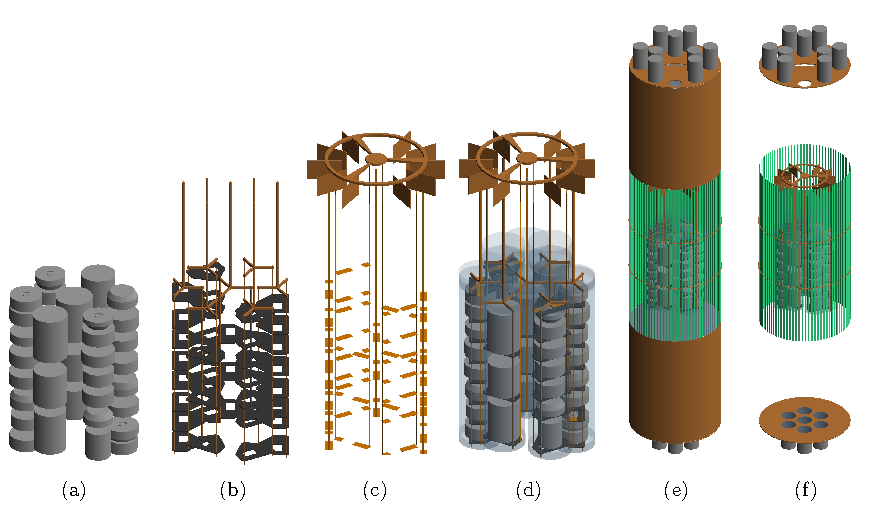
\includegraphics[width=\textwidth]{setup/mage-volumes.pdf}
  \caption{%
    Implementation of the \gerda\ array in \mage, visualized using the
    \geant\ visualization drivers. From left to right: a) the \gerda\
    detectors, b) the holder mounting, composed of silicon plates and
    copper bars c) the high-voltage and signal flexible flat cables plus
    the front-end electronics on top, d) the full array instrumentation,
    including the transparent nylon mini-shrouds, e) the full LAr veto
    system surrounding the array, including the fiber shroud (in green),
    the \tetratex-coated copper shrouds (above and below the fibers) and
    the two PMT arrays, f) the LAr veto system without the copper
    shrouds.%
  }\label{fig:setup:magevolumes}
\end{figure}

\section{Background reduction techniques}\label{sec:gerda:cuts}

Various background mitigation techniques are adopted, both at the data acquisition level
(online) and the analysis level (offline) in \gerda\ to lower the background index to the
`background-free' level of \pIIbi.

\marginnote{Muon veto}
As already described in \cref{sec:gerda:setup}, the \gerda\ muon veto comprises of a water
\v{C}erenkov veto and a scintillator veto.

% vim: tw=90
